\documentclass[twoside]{book}

% Packages required by doxygen
\usepackage{fixltx2e}
\usepackage{calc}
\usepackage{doxygen}
\usepackage[export]{adjustbox} % also loads graphicx
\usepackage{graphicx}
\usepackage[utf8]{inputenc}
\usepackage{makeidx}
\usepackage{multicol}
\usepackage{multirow}
\PassOptionsToPackage{warn}{textcomp}
\usepackage{textcomp}
\usepackage[nointegrals]{wasysym}
\usepackage[table]{xcolor}

% Font selection
\usepackage[T1]{fontenc}
\usepackage[scaled=.90]{helvet}
\usepackage{courier}
\usepackage{amssymb}
\usepackage{sectsty}
\renewcommand{\familydefault}{\sfdefault}
\allsectionsfont{%
  \fontseries{bc}\selectfont%
  \color{darkgray}%
}
\renewcommand{\DoxyLabelFont}{%
  \fontseries{bc}\selectfont%
  \color{darkgray}%
}
\newcommand{\+}{\discretionary{\mbox{\scriptsize$\hookleftarrow$}}{}{}}

% Page & text layout
\usepackage{geometry}
\geometry{%
  a4paper,%
  top=2.5cm,%
  bottom=2.5cm,%
  left=2.5cm,%
  right=2.5cm%
}
\tolerance=750
\hfuzz=15pt
\hbadness=750
\setlength{\emergencystretch}{15pt}
\setlength{\parindent}{0cm}
\setlength{\parskip}{0.2cm}
\makeatletter
\renewcommand{\paragraph}{%
  \@startsection{paragraph}{4}{0ex}{-1.0ex}{1.0ex}{%
    \normalfont\normalsize\bfseries\SS@parafont%
  }%
}
\renewcommand{\subparagraph}{%
  \@startsection{subparagraph}{5}{0ex}{-1.0ex}{1.0ex}{%
    \normalfont\normalsize\bfseries\SS@subparafont%
  }%
}
\makeatother

% Headers & footers
\usepackage{fancyhdr}
\pagestyle{fancyplain}
\fancyhead[LE]{\fancyplain{}{\bfseries\thepage}}
\fancyhead[CE]{\fancyplain{}{}}
\fancyhead[RE]{\fancyplain{}{\bfseries\leftmark}}
\fancyhead[LO]{\fancyplain{}{\bfseries\rightmark}}
\fancyhead[CO]{\fancyplain{}{}}
\fancyhead[RO]{\fancyplain{}{\bfseries\thepage}}
\fancyfoot[LE]{\fancyplain{}{}}
\fancyfoot[CE]{\fancyplain{}{}}
\fancyfoot[RE]{\fancyplain{}{\bfseries\scriptsize Generated on Fri Dec 4 2015 17\+:19\+:25 for Arnie\+Boids by Doxygen }}
\fancyfoot[LO]{\fancyplain{}{\bfseries\scriptsize Generated on Fri Dec 4 2015 17\+:19\+:25 for Arnie\+Boids by Doxygen }}
\fancyfoot[CO]{\fancyplain{}{}}
\fancyfoot[RO]{\fancyplain{}{}}
\renewcommand{\footrulewidth}{0.4pt}
\renewcommand{\chaptermark}[1]{%
  \markboth{#1}{}%
}
\renewcommand{\sectionmark}[1]{%
  \markright{\thesection\ #1}%
}

% Indices & bibliography
\usepackage{natbib}
\usepackage[titles]{tocloft}
\setcounter{tocdepth}{3}
\setcounter{secnumdepth}{5}
\makeindex

% Hyperlinks (required, but should be loaded last)
\usepackage{ifpdf}
\ifpdf
  \usepackage[pdftex,pagebackref=true]{hyperref}
\else
  \usepackage[ps2pdf,pagebackref=true]{hyperref}
\fi
\hypersetup{%
  colorlinks=true,%
  linkcolor=blue,%
  citecolor=blue,%
  unicode%
}

% Custom commands
\newcommand{\clearemptydoublepage}{%
  \newpage{\pagestyle{empty}\cleardoublepage}%
}


%===== C O N T E N T S =====

\begin{document}

% Titlepage & ToC
\hypersetup{pageanchor=false,
             bookmarks=true,
             bookmarksnumbered=true,
             pdfencoding=unicode
            }
\pagenumbering{roman}
\begin{titlepage}
\vspace*{7cm}
\begin{center}%
{\Large Arnie\+Boids \\[1ex]\large 0.\+0.\+1 }\\
\vspace*{1cm}
{\large Generated by Doxygen 1.8.10}\\
\vspace*{0.5cm}
{\small Fri Dec 4 2015 17:19:25}\\
\end{center}
\end{titlepage}
\clearemptydoublepage
\tableofcontents
\clearemptydoublepage
\pagenumbering{arabic}
\hypersetup{pageanchor=true}

%--- Begin generated contents ---
\chapter{Hierarchical Index}
\section{Class Hierarchy}
This inheritance list is sorted roughly, but not completely, alphabetically\+:\begin{DoxyCompactList}
\item Circle\+Shape\begin{DoxyCompactList}
\item \contentsline{section}{Star}{\pageref{class_star}}{}
\end{DoxyCompactList}
\item \contentsline{section}{Collision\+System}{\pageref{class_collision_system}}{}
\item Convex\+Shape\begin{DoxyCompactList}
\item \contentsline{section}{Bullet}{\pageref{class_bullet}}{}
\begin{DoxyCompactList}
\item \contentsline{section}{Missile}{\pageref{class_missile}}{}
\end{DoxyCompactList}
\item \contentsline{section}{Ship}{\pageref{class_ship}}{}
\begin{DoxyCompactList}
\item \contentsline{section}{Asteroid}{\pageref{class_asteroid}}{}
\item \contentsline{section}{Player}{\pageref{class_player}}{}
\item \contentsline{section}{Swarm\+Boid}{\pageref{class_swarm_boid}}{}
\end{DoxyCompactList}
\end{DoxyCompactList}
\item \contentsline{section}{Game}{\pageref{class_game}}{}
\item \contentsline{section}{Key\+Input}{\pageref{class_key_input}}{}
\item View\begin{DoxyCompactList}
\item \contentsline{section}{Camera}{\pageref{class_camera}}{}
\end{DoxyCompactList}
\item \contentsline{section}{X\+Controller}{\pageref{class_x_controller}}{}
\end{DoxyCompactList}

\chapter{Class Index}
\section{Class List}
Here are the classes, structs, unions and interfaces with brief descriptions\+:\begin{DoxyCompactList}
\item\contentsline{section}{\hyperlink{class_asteroid}{Asteroid} }{\pageref{class_asteroid}}{}
\item\contentsline{section}{\hyperlink{class_bullet}{Bullet} }{\pageref{class_bullet}}{}
\item\contentsline{section}{\hyperlink{class_camera}{Camera} }{\pageref{class_camera}}{}
\item\contentsline{section}{\hyperlink{class_collision_system}{Collision\+System} }{\pageref{class_collision_system}}{}
\item\contentsline{section}{\hyperlink{class_game}{Game} }{\pageref{class_game}}{}
\item\contentsline{section}{\hyperlink{class_key_input}{Key\+Input} }{\pageref{class_key_input}}{}
\item\contentsline{section}{\hyperlink{class_missile}{Missile} }{\pageref{class_missile}}{}
\item\contentsline{section}{\hyperlink{class_player}{Player} }{\pageref{class_player}}{}
\item\contentsline{section}{\hyperlink{class_ship}{Ship} \\*Base \hyperlink{class_ship}{Ship} class. Abstract class that inherits from sf\+::\+Convex\+Shape. Contains members common to all ships }{\pageref{class_ship}}{}
\item\contentsline{section}{\hyperlink{class_star}{Star} }{\pageref{class_star}}{}
\item\contentsline{section}{\hyperlink{class_swarm_boid}{Swarm\+Boid} }{\pageref{class_swarm_boid}}{}
\item\contentsline{section}{\hyperlink{class_x_controller}{X\+Controller} }{\pageref{class_x_controller}}{}
\end{DoxyCompactList}

\chapter{Class Documentation}
\hypertarget{class_game}{}\section{Game Class Reference}
\label{class_game}\index{Game@{Game}}


{\ttfamily \#include $<$Game.\+hpp$>$}

\subsection*{Public Member Functions}
\begin{DoxyCompactItemize}
\item 
\hypertarget{class_game_a50d0ebb6c8c0dbb762d2c1c10bc0c91c}{}{\bfseries Game} (unsigned int win\+Width=800\+U, unsigned int win\+Height=600\+U, unsigned int time\+Per\+Tick=16\+U)\label{class_game_a50d0ebb6c8c0dbb762d2c1c10bc0c91c}

\item 
\hypertarget{class_game_a99fb161fbbe87d25a8b73265a0611e58}{}int \hyperlink{class_game_a99fb161fbbe87d25a8b73265a0611e58}{run} ()\label{class_game_a99fb161fbbe87d25a8b73265a0611e58}

\begin{DoxyCompactList}\small\item\em Implements the main game loop. While window\+\_\+ is open\+: Calls handle\+Events(), Implements a fixed timestep and calls update() and draw() inside it. \end{DoxyCompactList}\end{DoxyCompactItemize}


\subsection{Detailed Description}
Updates and draws all ships and bullets. Culls dead bullets and ships.

\begin{DoxyRemark}{Remarks}
Chrono members are used for fixed timestep 
\end{DoxyRemark}


The documentation for this class was generated from the following files\+:\begin{DoxyCompactItemize}
\item 
Arnieboids/include/Game.\+hpp\item 
Arnieboids/src/Game.\+cpp\end{DoxyCompactItemize}

\hypertarget{class_player}{}\section{Player Class Reference}
\label{class_player}\index{Player@{Player}}
Inheritance diagram for Player\+:\begin{figure}[H]
\begin{center}
\leavevmode
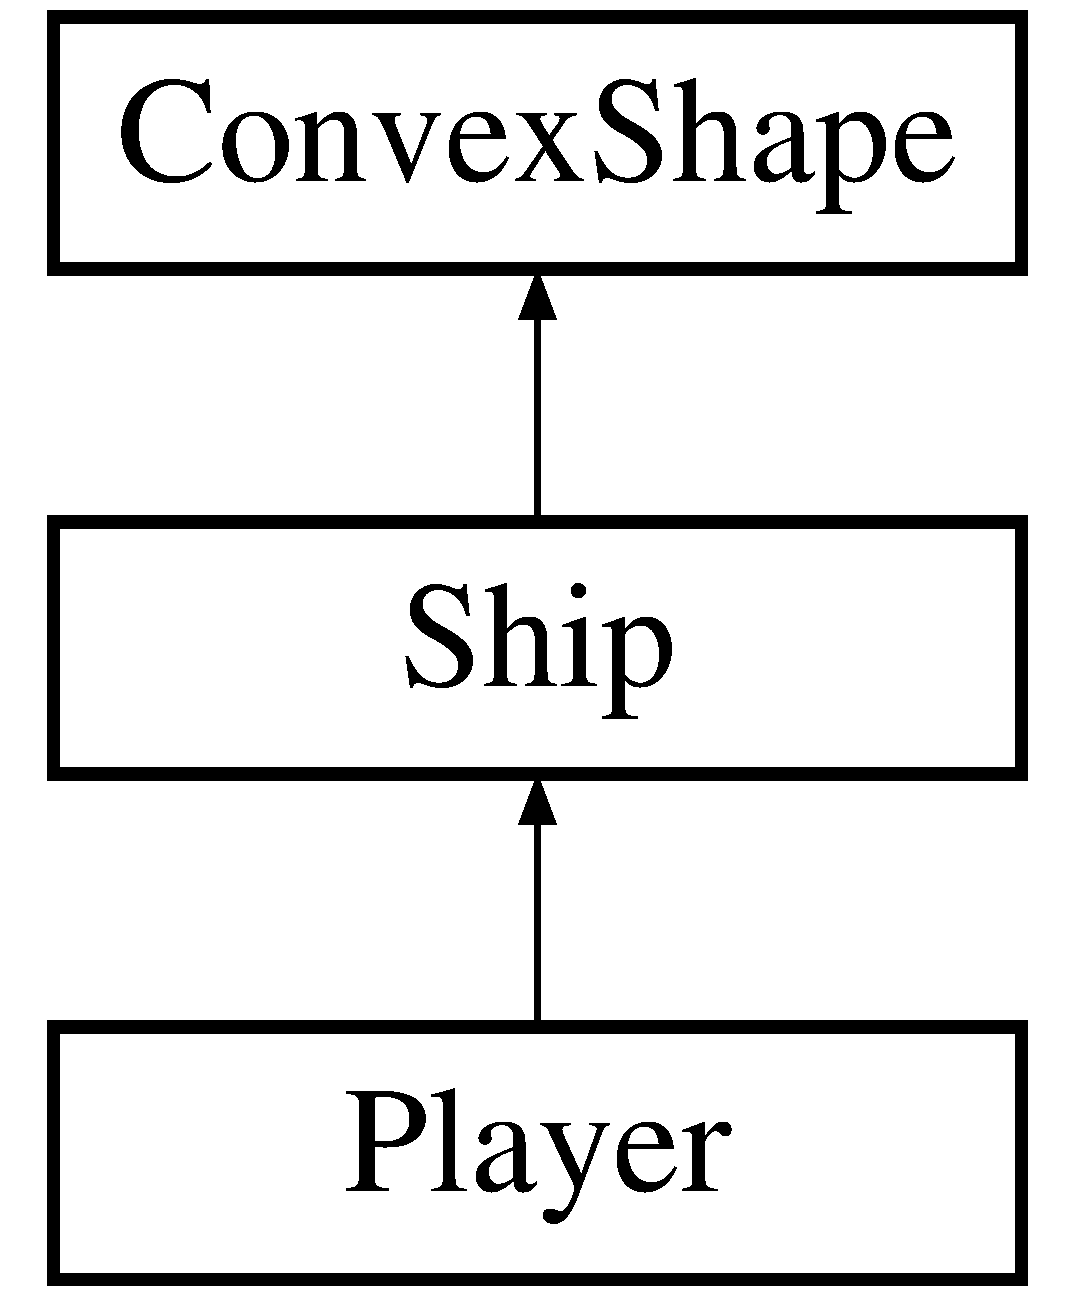
\includegraphics[height=2.000000cm]{class_player}
\end{center}
\end{figure}
\subsection*{Public Member Functions}
\begin{DoxyCompactItemize}
\item 
\hypertarget{class_player_aac1c48b82a1e579cae0f93482f1c6a22}{}{\bfseries Player} (sf\+::\+Vector2f const \&position, unsigned int max\+Health=10\+U)\label{class_player_aac1c48b82a1e579cae0f93482f1c6a22}

\item 
\hypertarget{class_player_a6912bb6e48efb5845d59f0f4582827ef}{}void \hyperlink{class_player_a6912bb6e48efb5845d59f0f4582827ef}{update} () override\label{class_player_a6912bb6e48efb5845d59f0f4582827ef}

\begin{DoxyCompactList}\small\item\em Hides sf\+::\+Shape\+::update() \end{DoxyCompactList}\end{DoxyCompactItemize}


The documentation for this class was generated from the following files\+:\begin{DoxyCompactItemize}
\item 
Arnieboids/include/Player.\+hpp\item 
Arnieboids/src/Player.\+cpp\end{DoxyCompactItemize}

\hypertarget{class_ship}{}\section{Ship Class Reference}
\label{class_ship}\index{Ship@{Ship}}


Base \hyperlink{class_ship}{Ship} class. Abstract class that inherits from sf\+::\+Convex\+Shape. Contains members common to all ships.  




{\ttfamily \#include $<$Ship.\+hpp$>$}

Inheritance diagram for Ship\+:\begin{figure}[H]
\begin{center}
\leavevmode
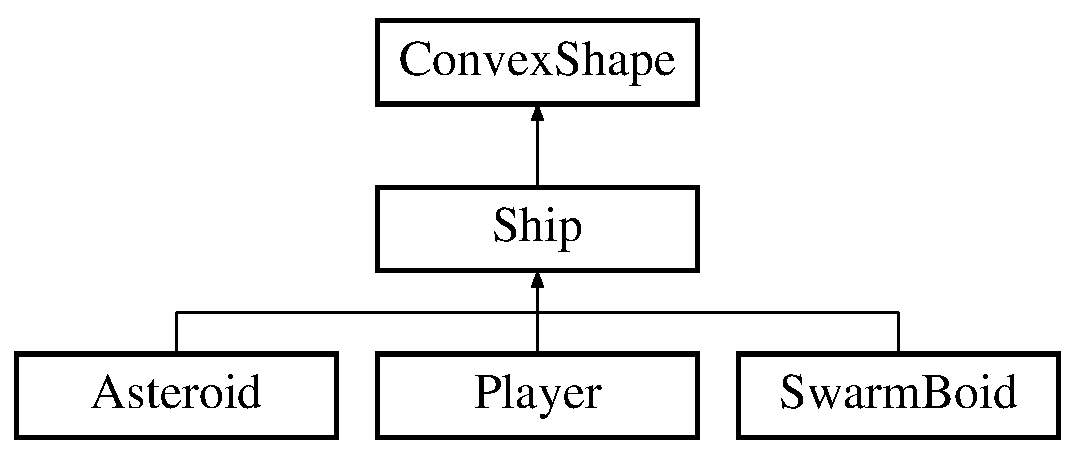
\includegraphics[height=3.000000cm]{class_ship}
\end{center}
\end{figure}
\subsection*{Public Member Functions}
\begin{DoxyCompactItemize}
\item 
\hypertarget{class_ship_a4361703fa6d49a17f080648e1c2dc60b}{}{\bfseries Ship} (float max\+Speed)\label{class_ship_a4361703fa6d49a17f080648e1c2dc60b}

\item 
\hypertarget{class_ship_abfe8b92e7f0346b198e8c40cff44ebeb}{}virtual void \hyperlink{class_ship_abfe8b92e7f0346b198e8c40cff44ebeb}{update} ()=0\label{class_ship_abfe8b92e7f0346b198e8c40cff44ebeb}

\begin{DoxyCompactList}\small\item\em Hides sf\+::\+Shape\+::update() \end{DoxyCompactList}\item 
\hypertarget{class_ship_a966830e20a179ada7d4b7301577b72d7}{}virtual void {\bfseries on\+Collide} (\hyperlink{class_ship}{Ship} $\ast$other)=0\label{class_ship_a966830e20a179ada7d4b7301577b72d7}

\item 
\hypertarget{class_ship_a3a0732b4bb4697b57398cec3b24d76ed}{}void {\bfseries take\+Damage} (unsigned int amount)\label{class_ship_a3a0732b4bb4697b57398cec3b24d76ed}

\item 
\hypertarget{class_ship_a52d219bbadbba6475b919f8e6497ce34}{}bool {\bfseries is\+Dead} () const \label{class_ship_a52d219bbadbba6475b919f8e6497ce34}

\end{DoxyCompactItemize}
\subsection*{Protected Member Functions}
\begin{DoxyCompactItemize}
\item 
\hypertarget{class_ship_a8e7bc2ee7d749ab0d28062091733987c}{}void \hyperlink{class_ship_a8e7bc2ee7d749ab0d28062091733987c}{clamp\+To\+Max\+Speed} ()\label{class_ship_a8e7bc2ee7d749ab0d28062091733987c}

\begin{DoxyCompactList}\small\item\em Clamps the length of the velocity\+\_\+ vector to M\+A\+X\+\_\+\+S\+P\+E\+E\+D\+\_\+. \end{DoxyCompactList}\end{DoxyCompactItemize}
\subsection*{Protected Attributes}
\begin{DoxyCompactItemize}
\item 
\hypertarget{class_ship_a6843554ddc3c0098bcc9d17f7a7fbf3b}{}const float \hyperlink{class_ship_a6843554ddc3c0098bcc9d17f7a7fbf3b}{M\+A\+X\+\_\+\+S\+P\+E\+E\+D\+\_\+}\label{class_ship_a6843554ddc3c0098bcc9d17f7a7fbf3b}

\begin{DoxyCompactList}\small\item\em Maximum length of velocity\+\_\+ vector. \end{DoxyCompactList}\item 
\hypertarget{class_ship_ac1584ef024d6ed1538eb2d1e99661557}{}sf\+::\+Vector2f \hyperlink{class_ship_ac1584ef024d6ed1538eb2d1e99661557}{velocity\+\_\+}\label{class_ship_ac1584ef024d6ed1538eb2d1e99661557}

\begin{DoxyCompactList}\small\item\em Change of position of ship per update. \end{DoxyCompactList}\item 
\hypertarget{class_ship_a6a377507ab7c9c91356869121a84c252}{}unsigned int {\bfseries health\+\_\+}\label{class_ship_a6a377507ab7c9c91356869121a84c252}

\end{DoxyCompactItemize}


\subsection{Detailed Description}
Base \hyperlink{class_ship}{Ship} class. Abstract class that inherits from sf\+::\+Convex\+Shape. Contains members common to all ships. 

The documentation for this class was generated from the following files\+:\begin{DoxyCompactItemize}
\item 
Arnieboids/include/Ship.\+hpp\item 
Arnieboids/src/Ship.\+cpp\end{DoxyCompactItemize}

\hypertarget{class_x_controller}{}\section{X\+Controller Class Reference}
\label{class_x_controller}\index{X\+Controller@{X\+Controller}}
\subsection*{Public Member Functions}
\begin{DoxyCompactItemize}
\item 
\hypertarget{class_x_controller_a148116f8235dd69b17f10c09ebc8e493}{}int {\bfseries get\+Port} () const \label{class_x_controller_a148116f8235dd69b17f10c09ebc8e493}

\item 
\hypertarget{class_x_controller_af065f53794859ac0664106a5ff024ef7}{}bool {\bfseries check\+Down} (W\+O\+R\+D button) const \label{class_x_controller_af065f53794859ac0664106a5ff024ef7}

\item 
\hypertarget{class_x_controller_a8f62325ebebceea3c56b164faf9c05cb}{}bool {\bfseries check\+Up} (W\+O\+R\+D button) const \label{class_x_controller_a8f62325ebebceea3c56b164faf9c05cb}

\item 
\hypertarget{class_x_controller_a1cc805edbaecf773f97bfcdbc77a2c4f}{}bool {\bfseries check\+Pressed} (W\+O\+R\+D button) const \label{class_x_controller_a1cc805edbaecf773f97bfcdbc77a2c4f}

\item 
\hypertarget{class_x_controller_a35587b82880720ea2b265d7a7d712190}{}bool {\bfseries check\+Released} (W\+O\+R\+D button) const \label{class_x_controller_a35587b82880720ea2b265d7a7d712190}

\item 
\hypertarget{class_x_controller_aa768bc43116edb8d33ffd4bc83f977fd}{}bool {\bfseries check\+Held} (W\+O\+R\+D button) const \label{class_x_controller_aa768bc43116edb8d33ffd4bc83f977fd}

\item 
\hypertarget{class_x_controller_ad8241a72453c9036b014e6c756bc4468}{}unsigned int {\bfseries check\+Time\+Held} (W\+O\+R\+D button) const \label{class_x_controller_ad8241a72453c9036b014e6c756bc4468}

\item 
\hypertarget{class_x_controller_a62f462d73f5264a0cb468c8d7b3e9da0}{}float {\bfseries check\+Left\+X} () const \label{class_x_controller_a62f462d73f5264a0cb468c8d7b3e9da0}

\item 
\hypertarget{class_x_controller_af78833f9a66c7422c8dd04c32ba35a86}{}float {\bfseries check\+Left\+Y} () const \label{class_x_controller_af78833f9a66c7422c8dd04c32ba35a86}

\item 
\hypertarget{class_x_controller_a99d1ca041e88e230253aaf069246502f}{}float {\bfseries check\+Right\+X} () const \label{class_x_controller_a99d1ca041e88e230253aaf069246502f}

\item 
\hypertarget{class_x_controller_a0eda1afa64aedd18caf7210dfd5fdf77}{}float {\bfseries check\+Right\+Y} () const \label{class_x_controller_a0eda1afa64aedd18caf7210dfd5fdf77}

\item 
\hypertarget{class_x_controller_a97ef1f5e2a9d1cb77f8ebbcdf05cacd9}{}bool {\bfseries check\+Left\+Neutral} () const \label{class_x_controller_a97ef1f5e2a9d1cb77f8ebbcdf05cacd9}

\item 
\hypertarget{class_x_controller_a6650c557d70250cf3b2def17ee068036}{}bool {\bfseries check\+Right\+Neutral} () const \label{class_x_controller_a6650c557d70250cf3b2def17ee068036}

\item 
\hypertarget{class_x_controller_a70320add88de714df1ecc235582d4647}{}int {\bfseries check\+D\+Pad\+X} () const \label{class_x_controller_a70320add88de714df1ecc235582d4647}

\item 
\hypertarget{class_x_controller_ac32d789c025f1eccebfb8edf08541c8f}{}int {\bfseries check\+D\+Pad\+Y} () const \label{class_x_controller_ac32d789c025f1eccebfb8edf08541c8f}

\item 
\hypertarget{class_x_controller_aa9360de1f75371dba977e6dbb9bf17c7}{}float {\bfseries check\+Left\+Trigger} () const \label{class_x_controller_aa9360de1f75371dba977e6dbb9bf17c7}

\item 
\hypertarget{class_x_controller_ab87836fe6d88d4af47f815e686ee4541}{}float {\bfseries check\+Right\+Trigger} () const \label{class_x_controller_ab87836fe6d88d4af47f815e686ee4541}

\item 
\hypertarget{class_x_controller_a59282aca9a7114e6bc64bc082f72fc53}{}bool {\bfseries check\+Left\+Hair\+Trigger} () const \label{class_x_controller_a59282aca9a7114e6bc64bc082f72fc53}

\item 
\hypertarget{class_x_controller_a691089784b0e48d6129235170c1256bb}{}bool {\bfseries check\+Right\+Hair\+Trigger} () const \label{class_x_controller_a691089784b0e48d6129235170c1256bb}

\item 
\hypertarget{class_x_controller_ae52c79dab419e0612bdf60494e9d9576}{}bool {\bfseries set\+Deadzone\+L\+X} (float deadzone)\label{class_x_controller_ae52c79dab419e0612bdf60494e9d9576}

\item 
\hypertarget{class_x_controller_aa993600f76d018dd7710edfd3da3430c}{}bool {\bfseries set\+Deadzone\+L\+Y} (float deadzone)\label{class_x_controller_aa993600f76d018dd7710edfd3da3430c}

\item 
\hypertarget{class_x_controller_a0d3993c8a609e8ea732db7b742ddf22e}{}bool {\bfseries set\+Deadzone\+R\+X} (float deadzone)\label{class_x_controller_a0d3993c8a609e8ea732db7b742ddf22e}

\item 
\hypertarget{class_x_controller_a4106c828fabe8a716f7109723776b5fa}{}bool {\bfseries set\+Deadzone\+R\+Y} (float deadzone)\label{class_x_controller_a4106c828fabe8a716f7109723776b5fa}

\item 
\hypertarget{class_x_controller_aa95c25f438c320aa455a1739191e9bb3}{}bool {\bfseries set\+Threshold\+L\+T} (float threshold)\label{class_x_controller_aa95c25f438c320aa455a1739191e9bb3}

\item 
\hypertarget{class_x_controller_a9fdc050189aa00d922b8101bc9bf5e5d}{}bool {\bfseries set\+Threshold\+R\+T} (float threshold)\label{class_x_controller_a9fdc050189aa00d922b8101bc9bf5e5d}

\item 
\hypertarget{class_x_controller_ab00ba988d215a523a7730f20594fa2c5}{}float {\bfseries get\+Deadzone\+L\+X} () const \label{class_x_controller_ab00ba988d215a523a7730f20594fa2c5}

\item 
\hypertarget{class_x_controller_a705a1d4ad575e6ef15db2391813fd18e}{}float {\bfseries get\+Deadzone\+L\+Y} () const \label{class_x_controller_a705a1d4ad575e6ef15db2391813fd18e}

\item 
\hypertarget{class_x_controller_a08bf17b0a3c086bf5667cf3286cbc585}{}float {\bfseries get\+Deadzone\+R\+X} () const \label{class_x_controller_a08bf17b0a3c086bf5667cf3286cbc585}

\item 
\hypertarget{class_x_controller_abb171d26892efcc9ef5d4109a0e46644}{}float {\bfseries get\+Deadzone\+R\+Y} () const \label{class_x_controller_abb171d26892efcc9ef5d4109a0e46644}

\item 
\hypertarget{class_x_controller_a29521bc4c619301d8448cd9b1fa84bc4}{}float {\bfseries get\+Threshold\+L\+T} () const \label{class_x_controller_a29521bc4c619301d8448cd9b1fa84bc4}

\item 
\hypertarget{class_x_controller_a74406c5161e85934a0a25a11ca44fa96}{}float {\bfseries get\+Threshold\+R\+T} () const \label{class_x_controller_a74406c5161e85934a0a25a11ca44fa96}

\item 
\hypertarget{class_x_controller_addafe067b836a5b5d6cfa6a1d9ff72cb}{}bool {\bfseries update} (int milliseconds)\label{class_x_controller_addafe067b836a5b5d6cfa6a1d9ff72cb}

\end{DoxyCompactItemize}


The documentation for this class was generated from the following files\+:\begin{DoxyCompactItemize}
\item 
Arnieboids/include/X\+Controller.\+hpp\item 
Arnieboids/src/X\+Controller.\+cpp\end{DoxyCompactItemize}

%--- End generated contents ---

% Index
\backmatter
\newpage
\phantomsection
\clearemptydoublepage
\addcontentsline{toc}{chapter}{Index}
\printindex

\end{document}
